\documentclass[12pt, letterpaper]{article}
\usepackage[utf8]{inputenc}
\usepackage{enumitem}
\usepackage{amsmath}
\usepackage{tikz}
\usepackage{subcaption}
\usepackage{float}

\usetikzlibrary{arrows}

\title{Assisgnment 1, TDT4171}
\author{Martin Bjerke}

\begin{document}
\maketitle


\section{5-card Poker Hands}

\begin{enumerate}[label=(\alph*)]
  \item The total number of possible 5-card hands are $\binom{52}{5} = 2598960$
    (number of atomic events)
  \item Since the dealer is fair, each atomic event has an equal probability, $P
    = \frac{1}{2598960} = 3.85 \cdot 10^{-7} $
  \item As there are only 4 possible combinations of a royal straight flushsuit(one
    for each suit) $P(RSF) = 4 \cdot \frac{1}{2598960} = 1.54 \cdot 10^{-6} $
    and there are 13 possible four of a kind, with the last card(one of 48) does
    not matter $P(FOK) = 13 \cdot \cdot 48 \frac{1}{2598960} = 2.40 \cdot 10^{-4} $.
\end{enumerate}

\section{Bayesian Network Construction}

\begin{figure}[ht]
  \centering
  \begin{subfigure}[b]{ 0.3\textwidth }

    \centering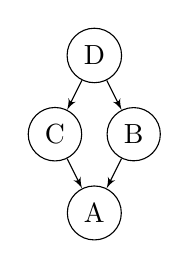
\begin{tikzpicture}
      \tikzset { vertex/.style = { shape=circle,draw,minimum size=1.5em } }
      \tikzset { edge/.style = { ->,> = latex' } }

      \node[vertex] (a) at (0.5,0) {A};
      \node[vertex] (b) at (1,1) {B};
      \node[vertex] (c) at (0,1) {C};
      \node[vertex] (d) at (0.5,2) {D};

      \draw[edge] (d) to (b);
      \draw[edge] (d) to (c);
      \draw[edge] (b) to (a);
      \draw[edge] (c) to (a);

    \end{tikzpicture}
    \caption{Problem 1}
  \end{subfigure}
  \begin{subfigure}[b]{0.3\textwidth}

    \centering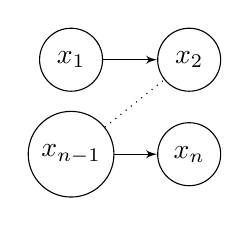
\begin{tikzpicture}
      \tikzset { vertex/.style = { shape=circle,draw,minimum size=0.8cm } }
      \tikzset { edge/.style = { ->,> = latex' } }

      \node[vertex] (a) at (1.5,0) {$x_n$};
      \node[vertex] (b) at (0,0) {$x_{n-1}$};
      \node[vertex] (c) at (1.5,1.2) {$x_2$};
      \node[vertex] (d) at (0,1.2) {$x_1$};

      \draw[dotted] (b) to (c);
      \draw[edge] (d) to (c);
      \draw[edge] (b) to (a);

    \end{tikzpicture}
    \caption{Problem 2}
  \end{subfigure}
  \begin{subfigure}[b]{0.3\textwidth}

    \centering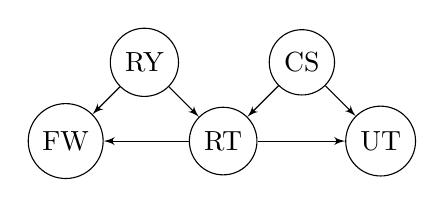
\begin{tikzpicture}
      \tikzset { vertex/.style = { shape=circle,draw,minimum size=1.5em } }
      \tikzset { edge/.style = { ->,> = latex' } }

      \node[vertex] (a) at (0,0) {FW};
      \node[vertex] (b) at (1,1) {RY};
      \node[vertex] (c) at (2,0) {RT};
            \node[vertex] (d) at (3,1) {CS};
      \node[vertex] (e) at (4,0) {UT};

      \draw[edge] (b) to (a);
      \draw[edge] (b) to (c);
      \draw[edge] (c) to (a);
      \draw[edge] (c) to (e);
      \draw[edge] (d) to (c);
      \draw[edge] (d) to (e);

    \end{tikzpicture}
    \caption{Problem 3}
  \end{subfigure}

\end{figure}

\subsection{Problem 1}

The complete network would have a CPT with $2^4-1 = 15$ entries, but using
the indepence structure this can be reduced to only $2^0+2^1+2^1+2^2 = 9$ entries.

\begin{figure}[H]
  \begin{subfigure}[t]{0.14\textwidth}
    \begin{tabular}[t]{|c|}
      \hline
      P(D) \\
      \hline
      0.9 \\
      \hline
    \end{tabular}
  \end{subfigure}
  \begin{subfigure}[t]{0.2\textwidth}
    \begin{tabular}[t]{|c|c|}
      \hline
      D & P(C) \\
      \hline
      t & 0.6 \\
      f & 0.5 \\
      \hline
    \end{tabular}
  \end{subfigure}
  \begin{subfigure}[t]{0.2\textwidth}
    \begin{tabular}[t]{|c|c|}
      \hline
      D & P(B) \\
      \hline
      t & 0.5 \\
      f & 0.6 \\
      \hline
    \end{tabular}
  \end{subfigure}
  \begin{subfigure}[t]{0.4\textwidth}
    \begin{tabular}[t]{|c|c|c|}
      \hline
      B & C & P(A) \\
      \hline
      t & t & 0.1 \\
      t & f & 0.2 \\
      f & t & 0.3 \\
      f & f & 0.4 \\
      \hline
    \end{tabular}
  \end{subfigure}

\end{figure}

\subsection{Problem 2}

The complete network would have a CPT with $2^n-1$ entries, but using
the indepence structure this can be reduced to only
$2^0+2^1+2^1+...+2^1 = 2^0 + (n-1)2^1$ entries.

\begin{figure}[H]
  \begin{subfigure}[t]{0.14\textwidth}
    \begin{tabular}[t]{|c|}
      \hline
      P($X_1$) \\
      \hline
      0.9 \\
      \hline
    \end{tabular}
  \end{subfigure}
  \begin{subfigure}[t]{0.2\textwidth}
    \begin{tabular}[t]{|c|c|}
      \hline
      $X_1$ & P($X_2$) \\
      \hline
      t & 0.8 \\
      f & 0.7 \\
      \hline
    \end{tabular}
  \end{subfigure}
  \begin{subfigure}[t]{0.17\textwidth}
    \begin{tabular}[t]{|c|c|}
      \hline
      $X_2$ & P($X_3$) \\
      \hline
      t & 0.8 \\
      f & 0.7 \\
      \hline
    \end{tabular}
  \end{subfigure}
  \begin{subfigure}{0.06\textwidth}
    \begin{tabular}{c}
      \\
      \\
      \\
      \\
      $\cdots$ \\
    \end{tabular}
  \end{subfigure}
  \begin{subfigure}[t]{0.35\textwidth}
    \begin{tabular}[t]{|c|c|}
      \hline
      $X_{n-1}$ & P($X_n$) \\
      \hline
      t & 0.1 \\
      f & 0.2 \\
      \hline
    \end{tabular}
  \end{subfigure}

\end{figure}

\subsection{Problem 3}

The complete network would have a CPT with $2^5-1 = 31$ entries, but using
the indepence structure this can be reduced to only $2^0+2^0+2^2+2^2+2^2 = 14$ entries.

\begin{figure}[H]
  \begin{subfigure}[t]{0.5\textwidth}
    \centering\begin{tabular}[ct]{|c|}
      \hline
      P(RY) \\
      \hline
      0.9 \\
      \hline
    \end{tabular}
  \end{subfigure}
  \begin{subfigure}[t]{0.5\textwidth}
    \begin{tabular}[ct]{|c|}
      \hline
      P(CS) \\
      \hline
      0.8 \\
      \hline
    \end{tabular}
  \end{subfigure}
  \begin{subfigure}[t]{0.3\textwidth}
    \begin{tabular}[t]{|c|c|c|}
      \hline
      RY & RT & P(FW) \\
      \hline
      t & t & 0.1 \\
      t & f & 0.2 \\
      f & t & 0.3 \\
      f & f & 0.4 \\
      \hline
    \end{tabular}
  \end{subfigure}
  \begin{subfigure}[t]{0.3\textwidth}
    \begin{tabular}[t]{|c|c|c|}
      \hline
      CS & RY & P(RT) \\
      \hline
      t & t & 0.2 \\
      t & f & 0.3 \\
      f & t & 0.5 \\
      f & f & 0.7 \\
      \hline
    \end{tabular}
  \end{subfigure}
  \begin{subfigure}[t]{0.3\textwidth}
    \begin{tabular}[t]{|c|c|c|}
      \hline
      CS & RT & P(UT) \\
      \hline
      t & t & 0.15 \\
      t & f & 0.22 \\
      f & t & 0.36 \\
      f & f & 0.48 \\
      \hline
    \end{tabular}
  \end{subfigure}


\end{figure}

\section{Bayesian Network Application}

\begin{figure}[ht]
  \centering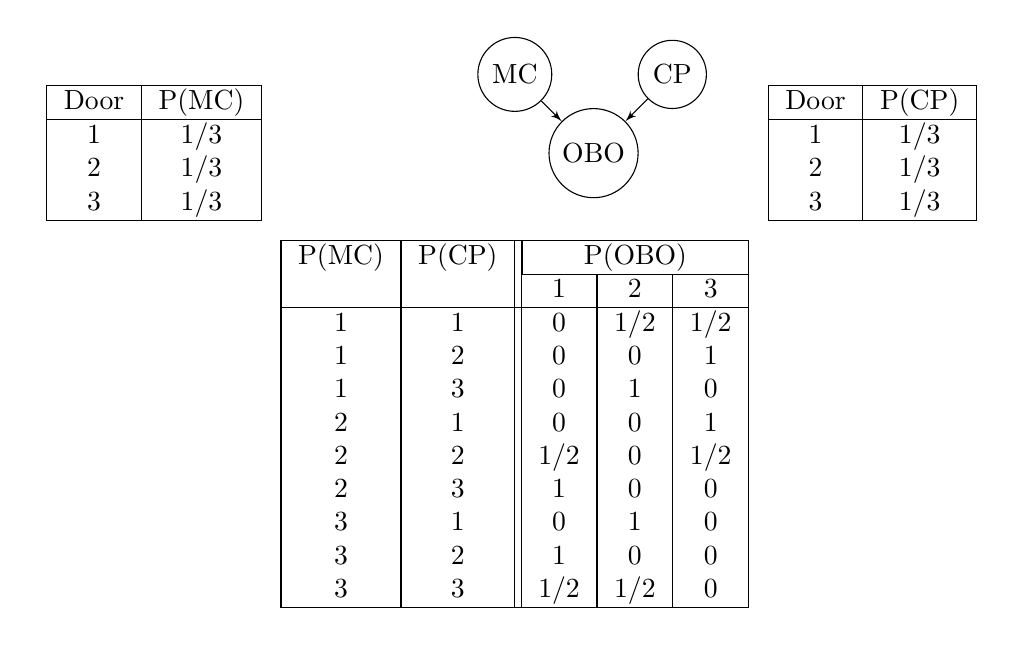
\begin{tikzpicture}
    \tikzset { vertex/.style = { shape=circle,draw,minimum size=1.5em } }
    \tikzset { edge/.style = { ->,> = latex' } }

    \matrix[ampersand replacement=\&] {
      \node (cptMC) [shape=rectangle] {
        \begin{tabular}{|c|c|}
          \hline
          Door & P(MC)\\
          \hline
          1 & 1/3 \\
          2 & 1/3 \\
          3 & 1/3 \\
          \hline
        \end{tabular}
      };

      \&

      \node[vertex] (a) at (1,0) {OBO};
      \node[vertex] (b) at (2,1) {CP};
      \node[vertex] (c) at (0,1) {MC};

      \draw[edge] (b) to (a);
      \draw[edge] (c) to (a);

      \&

      \node (cptCP) [shape=rectangle] {
        \begin{tabular}{|c|c|}
          \hline
          Door & P(CP)\\
          \hline
          1 & 1/3 \\
          2 & 1/3 \\
          3 & 1/3 \\
          \hline
        \end{tabular}
      }; \\

      \&

      \node (cptMC) [shape=rectangle] {
        \begin{tabular}{|c|c||c|c|c|}
          \hline
          P(MC) & P(CP) & \multicolumn{3}{|c|}{P(OBO)} \\
          \cline{3-5}
           & & 1 & 2 & 3 \\
          \hline
          1 & 1 & 0 & 1/2 & 1/2 \\
          1 & 2 & 0 & 0 & 1 \\
          1 & 3 & 0 & 1 & 0 \\
          2 & 1 & 0 & 0 & 1 \\
          2 & 2 & 1/2 & 0 & 1/2 \\
          2 & 3 & 1 & 0 & 0 \\
          3 & 1 & 0 & 1 & 0 \\
          3 & 2 & 1 & 0 & 0 \\
          3 & 3 & 1/2 & 1/2 & 0 \\
          \hline
        \end{tabular}
      }; \\
    };

  \end{tikzpicture}
  \caption{MC - MyChoice, CP - ContainsPrize, OBO - OpenedByOfficial}

\end{figure}

Throughout the game the probabilities change in the following way:
\begin{enumerate}
\item First I choose a door with the probability of a prize beeing behind it
  P(prize) = 1/3.
\item Then the official chooses a door with no prize behind it. The probability
  of which door he chooses is shown in the above CPT. Summarising, 1/3 of the
  time he can choose between 2 doors, each beeing equally possible, and the
  other 2/3 of the time he can only choose one door.
  \item Now the probability of the prize beeing behind the door I choose first
    is 1/3 and the other door has a probability of 2/3 of having a prize behind it.
\end{enumerate}

The above CPT for P(OBO) show all the probabilities of which doors the official
opens, given the door I choose and the door the money price is behind. From the
table it is easy to see that in only 1/3 of the possible outcomes the prize is
behind the door I first choose. In the other 2/3 of the possible outcomes
I will have choosen a door without a prize behind it. The official will then
remove another door with no prize behind it and I will be guarnteed a prize if I
change to the last door. Totaling in a probability of 2/3 of me getting a prize
if I change to the other door after the official opens one door.


\end{document}
